\part{windows}

%%%%%%%%%%%%%%%%%%%%%%%%%%%%%%%%%%%%%%%%%%%%%%%%%%%%%%%%%%%%%%%%%%%%%%%%%%%
\begin{frame}[fragile]
  \frametitle{Some remarks}
  \framesubtitle{FYI}

  Keep in mind:
  \begin{itemize}
    \item You have \textit{root} access to your virtual machines
    \item Your virtual machines are often visible from the Internet
    \item It is up to you to keep your virtual machines updated and secure
    \item \textbf{DO NOT USE} password-based authentication for remote access
    \item You should terminate your virtual machine as soon as it is not
          needed anymore
    \item cloud-init is NOT configuration management!
  \end{itemize}

\end{frame}


%%%%%%%%%%%%%%%%%%%%%%%%%%%%%%%%%%%%%%%%%%%%%%%%%%%%%%%%%%%%%%%%%%%%%%%%%%%

\begin{frame}
  \frametitle{Prepare your own images}
  \framesubtitle{Install image}
    
  \begin{block}{Create your image}
    \begin{itemize}
        \item Install your OS:
        \begin{itemize}
            \item try to keep image size small, no need to store 0s
            \item any partition schema should work, I personally use a
                single / partition, no swap, nor /boot.
        \end{itemize}
        \item Install cloud-init (v0.7.5 fully supports all FedCloud RP)
        \item Disable root password: \texttt{passwd -d root}
        \item Clean-up hardware details (e.g. network devices):
        \begin{itemize}
            \item Manually: remove \texttt{/etc/udev/rules.d/70-persistent-net.rules}
            \item With \texttt{virt-sysprep}
        \end{itemize}
    \end{itemize}
  \end{block}
\end{frame}

%%%%%%%%%%%%%%%%%%%%%%%%%%%%%%%%%%%%%%%%%%%%%%%%%%%%%%%%%%%%%%%%%%%%%%%%%%%

\begin{frame}
  \frametitle{Prepare your own images}
  \framesubtitle{Convert to OVA}
    
  \begin{block}{Convert to OVA}
    \begin{itemize}
        \item FedCloud promotes the use of \texttt{OVA} packages.
        \begin{itemize}
        \item Contains a \texttt{OVF} file that describes the image.
        \item and a set of disk files.
        \end{itemize}
        \item VirtualBox does support exporting to \texttt{OVA} directly.
        \item See https://github.com/enolfc/img-tools/ if you are using KVM/Xen.
    \end{itemize}
  \end{block}
\end{frame}

%%%%%%%%%%%%%%%%%%%%%%%%%%%%%%%%%%%%%%%%%%%%%%%%%%%%%%%%%%%%%%%%%%%%%%%%%%%

\begin{frame}
  \frametitle{Prepare your own images}
  \framesubtitle{Upload to AppDB}

  \begin{block}{Upload to AppDB}
    \begin{itemize}
        \item A cloud-init script (user-data) can be attached to a VM
            in AppDB.
    \end{itemize}
    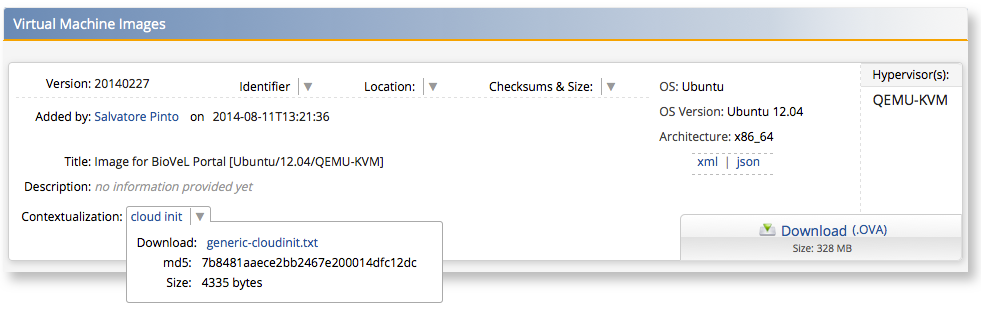
\includegraphics[width=\textwidth]{images/appdb_context}

  \end{block}
\end{frame}

